% !TeX encoding=utf-8
\documentclass[a4paper]{feidipsp}
\usepackage[pdftex]{graphicx}
\DeclareGraphicsExtensions{.pdf}
\graphicspath{{figures/}}

\usepackage[slovak]{babel}
\usepackage[utf8]{inputenc}
\usepackage[T1]{fontenc}
\usepackage{lmodern}

\usepackage{amsmath,amsfonts,amssymb,latexsym}

\def\figurename{Obrázok}
\def\tabname{Tabuľka}

%\usepackage[dvips]{graphicx}
%\DeclareGraphicsExtensions{.eps}

%\usepackage[pdftex]{hyperref}   %% tlac !!!
\usepackage[pdftex,colorlinks,citecolor=magenta,bookmarksnumbered,unicode,pdftoolbar=true,pdfmenubar=true,pdfwindowui=true,bookmarksopen=true]{hyperref}
\hypersetup{%
baseurl={http://www.tuke.sk/sevcovic},
pdfcreator={pdfcsLaTeX},
pdfkeywords={Sytémová príručka},
pdftitle={Šablóna na písanie DP na FEI TU v~Košiciach},
pdfauthor={Ján Buša, Ladislav Ševčovič},
pdfsubject={Ako napísať peknú DP}
}

% Citovanie podla mena autora a roku
%\usepackage[numbers]{natbib}
\usepackage{natbib} \citestyle{chicago}

%\usepackage{mathptm} %\usepackage{times}

\katedra{Laboratórium priemyselného inžinierstva}
\department{Laboratory of Industrial Engineering}
\odbor{Experimentálna fyzika}
\autor{Ján Zelený}
\veduci{Doc.~Ing.~Vojtech Čierny, CSc.}
\konzultant{Ing. Matej Biely, PhD.}
\nazov{Optimalizácia písania diplomových prác na našej fakulte}
\kratkynazov{Optimalizácia písania DP}
\nazovprogramu{ODYSSEUS}
\klucoveslova{optimalizácia, diplomová práca, písanie}
\title{The optimization of the diploma writing at our faculty}
\keywords{optimization, diploma, writing}
\datum{1. 4. 2004}



\begin{document}
\bibliographystyle{dcu}

\titulnastrana

\tableofcontents

\newpage

\setcounter{page}{1}

\section{Funkcia programu}

Krátky popis funkcie navrhovaného programu.

\section{Analýza riešenia}

Analýza riešeného problému včítane teoretického rozboru, porovnanie koncepcii možných
riešení, zdôvodnenie zvoleného postupu riešenia a~pod.

\section{Popis programu}

Maximálne využívat formálne a~grafické prostriedky podla použitej metodológie návrhu.
Je potrebné urobit odvolávky na zdrojové texty uvedené v~prílohách dokumentácie. Popis
castí podprogramov môže byt prebraný  z~komentárov uvedených v~zdrojových textov
programov. Hlavné komentáre (celoriadkové) musia odpovedat textovému popisu hrubého 
algoritmu riešenia.

V~texte môžu byt použité obrázky a~tabulky podla nasledujúcich príkladov:

\begin{figure}[!ht]
\centering 
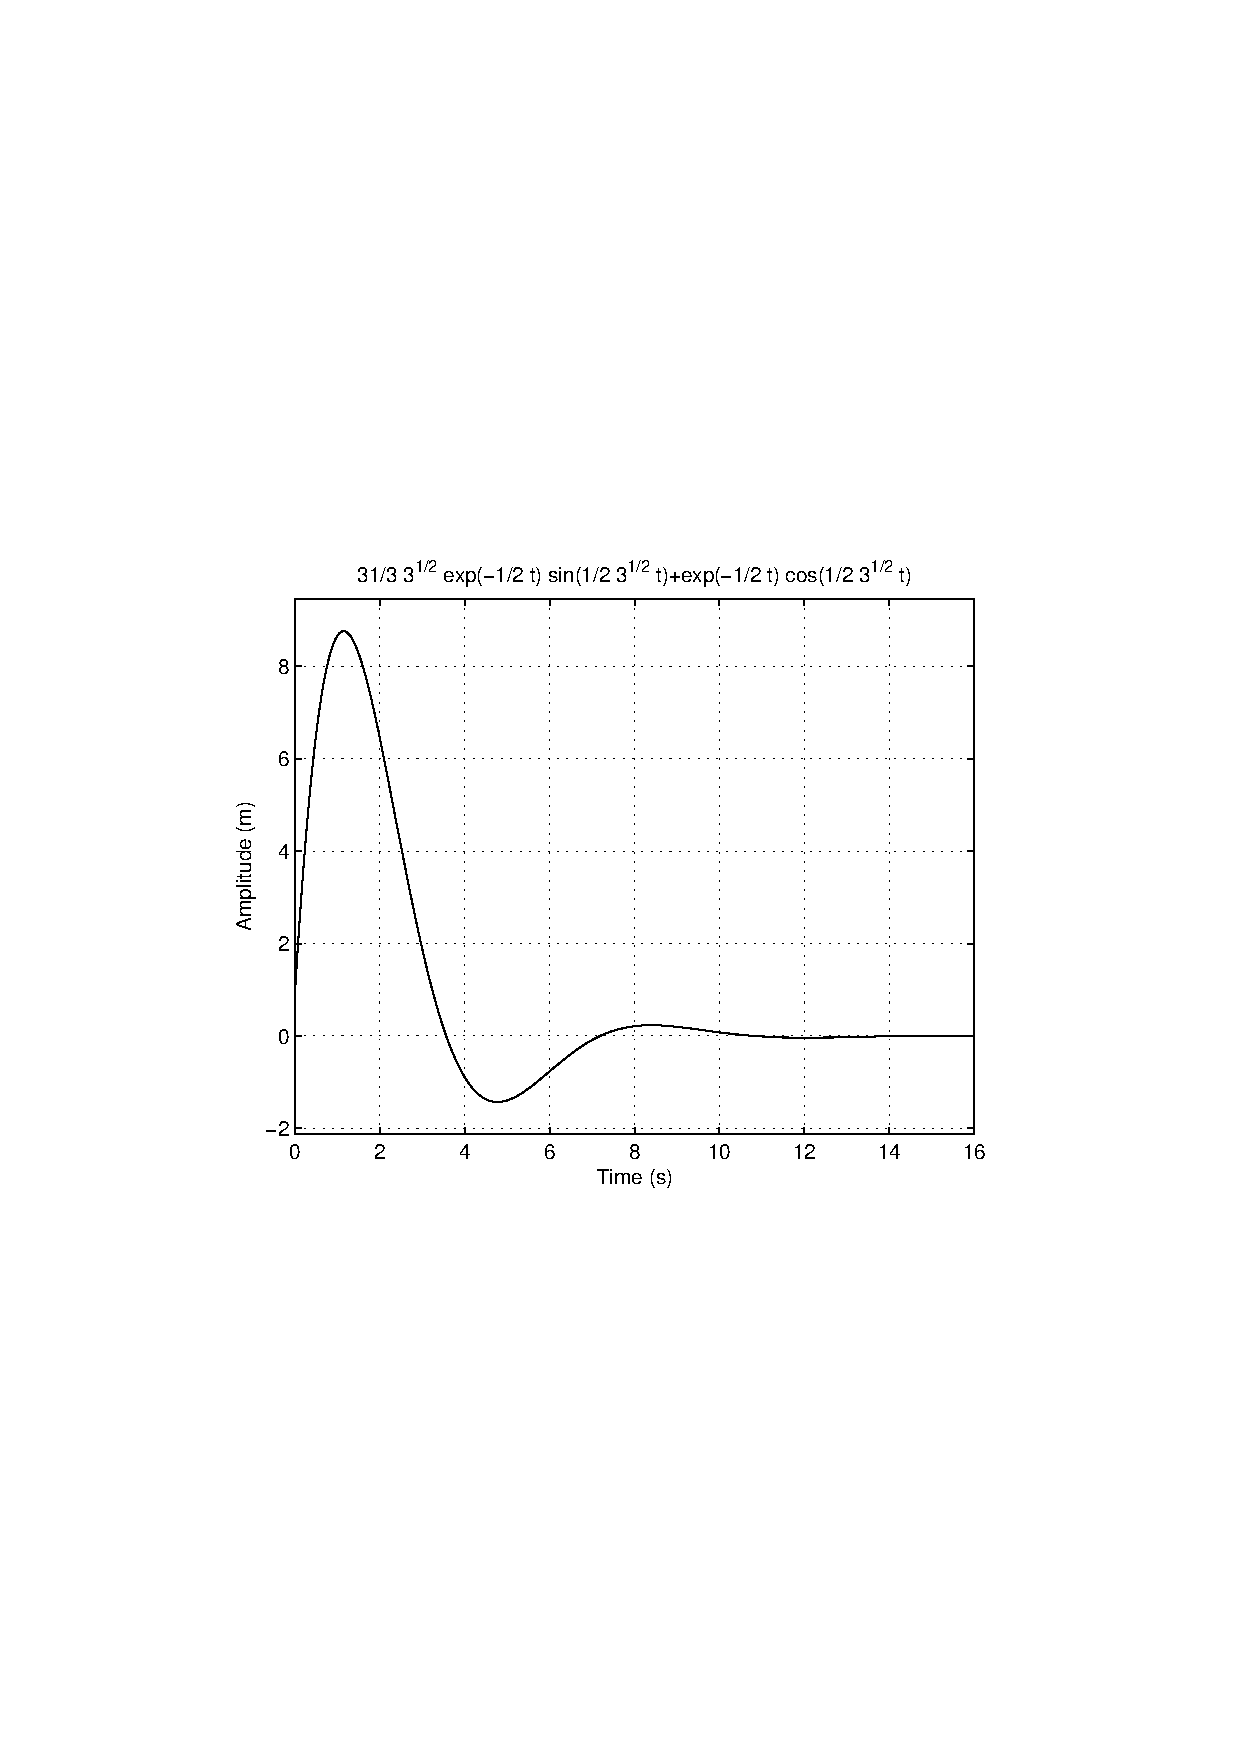
\includegraphics[width=0.5\textwidth]{tlmosc}
\caption{Tlmené oscilácie}\label{o:1}
\end{figure}

Obrázok by mal byt podla možnosti centrovaný. Pri jeho popisovaní v~texte treba použit odkazy na obrázok v~tvare obrázok \ref{o:1}  (kapitola 3, obrázok 1).

\begin{table}[!ht]\caption{Prehľad jednotiek}\label{t:1}
\smallskip
\centering
\begin{tabular}{|l|c|} \hline
Názov	& [\,jednotka] \\ \hline
Napätie & $\mu$V \\ \hline
\end{tabular}	
\end{table}


Tabulka by mala byť podla možnosti centrovaná. Pri jej popisovaní v~texte treba použiť odkazy na tabuľku v~tvare tabuľka \ref{t:1} (kapitola 3, tabuľka 1).

Na číslovanie obrázkov, resp. tabuliek treba použit desatinné triedenie, prvé číslo odpovedá číslu kapitoly resp. podkapitoly.


\subsection{Popis riešenia}

Uviesť teoretický základ resp koncepciu riešenia, použité vzťahy a~pod. s~odvolaním sa na literatúru uvedenú v~záverečnej kapitole

\subsection[Popis  algoritmov a~údajových štruktúr, globálnych premenných]{Popis  algoritmov a~údajových štruktúr, globálnych\\ premenných}

Popis algoritmov uviest s~použitím vhodných formálnych prostriedkov (vývojový diagram, verbálny popis atd.).podla použitej metodológie návrhu.

Popis návrhu dialógu s~používatelom. 

\subsection{Popis modulov a~podprogramov}

U~podprogramov uviest funkciu, popis vstupných a~výstupných parametrov, globálne premenné, ktoré používa, uviest popis algoritmu. Znázornit v~grafickej forme spôsob vnorenia volaní podprogramov.

\subsection{Popis vstupných a~výstupných súborov}

Pokial existujú. Popis charakter vstupu, organizáciu a~pokyny pre predprípravu  vstupných údajov.

\section{Preklad programu}

Popis prekladu programu.

\subsection{Zoznam zdrojových textov}

Zoznam s~odvolaním sa na prílohy.

\subsection{Požiadavky na technické prostriedky pri preklade}

Typ potrebného pocítaca, potrebná velkost operacnej pamäte, diskový priestor, prídavné zariadenia, atd.

\subsection{Požiadavky na programové prostriedky pri preklade}

Operacný systém, typ prekladaca a~spojovacieho programu, atd.

\subsection{Vlastný preklad}

Popis príkazových súborov a~pod., popis  nastavenia, konfigurácie prostredia, v~ktorom bol program vyvíjaný.

\section{Náväznost na iné programové produkty}

Napr. program môže využívat programový systém GKS, OpenGL, atď.

\section{Zhodnotenie riešenia}

Čo je nedopracované, možnosti dalšieho vývoja, obmedzenia riešenia, existujúce okolnosti riešenia, atď.

\section{Zoznam použitej literatúry}

Odkazy na použitú literatúru sa realizujú takým istým spôosobom ako v~texte hlavnej cast diplomovej práce, napr.

\def\refname{Zoznam použitej literatúry}
\addcontentsline{toc}{section}{\numberline{}Zoznam použitej literatúry}

\begin{thebibliography}{999}
\harvarditem{Barancok et al.}{1995}{barancok}
BARANCOK, D. et al. 1995. \emph{The effect of semiconductor surface treatment on LB film/Si interface.} In:~Physica Status Solidi /a/,  ISSN 0031-8965, 1995, vol. 108, no.2, pp. K~87\,--\,90

\harvarditem{Gonda}{2001}{gonda}
GONDA, V. 2001. \emph{Ako napísať a~úspešne obhájiť diplomovú prácu.} Bratislava : Elita, 2001, 3.~doplnené a~prepracované vydanie, 120~s. ISBN 80-8044-075-1

\harvarditem{Jadr. fyz. a~tech.}{1985}{slovnik}
\emph{Jadrová fyzika a~technika: Terminologický výkladový slovník.} 2.~rev.~vyd. Bratislava : ALFA, 1985. 235 s. ISBN 80-8256-030-5

\harvarditem{Katušcák}{1998}{kat}
KATUŠČÁK, D. \emph{Ako písať vysokoškolské a~kvalifikačné práce.} Bratislava : Stimul, 1998, 2.~doplnené vydanie. 121~s. ISBN 80-85697-82-3


\harvarditem{Lamoš a~Potocký}{1989}{lamos}
LAMOŠ, F. -- POTOCKÝ, R. 1989. \emph{Pravdepodobnosť a~matematická štatistika.} 1.~vyd. Bratislava : Alfa, 1989. 344 s. ISBN 80-8046-020-5

\harvarditem{PASC-L}{1989}{pasc} PASC-L (Public Access Computer Systems Forum). [online]. Houston : University of Houston Libraries. June 1989. [cit: 1995-05-07]. Dostupné na internete: \verb+<listserv@uhupvm.uh.edu>+

\harvarditem{Sýkora a~i.}{1980}{sykora}
SÝKORA, F. a~iní. 1980. \emph{Telesná výchova a~šport.} 1.~vyd. Bratislava : SPN, 1980. 35 s. ISBN 80-8046-020-5


\end{thebibliography}



\section{Zoznam príloh}

Prílohy obsahujú výpisy zdrojových textov programov. Každý zdrojový text zacína s~komentárovou hlavickou obsahujúcou nasledujúce informácie:

Súbor: názov súboru

Program: názov programu

Vypracoval:  meno diplomanta

Diplomová práca: názov diplomovej práce

Vedúci diplomovej práce: meno vedúceho diplomovej práce

Konzultant(i): meno konzultanta c.1, meno konzultanta c.2

\addcontentsline{toc}{section}{\numberline{}Zoznam obrázkov}
\listoffigures

\addcontentsline{toc}{section}{\numberline{}Zoznam tabuliek}
\listoftables



\end{document}
